% ============================================================
% Poster diagrams for the DJ track recommendation project
%
% Compile:  pdflatex poster_assets.tex
% Each tikzpicture environment becomes its own cropped PDF page
% (standalone class with multi=tikzpicture). Crop or screenshot any
% page directly into the poster.
%
% Choices made where the spec was open:
%  - sans-serif body via helvet for poster aesthetic; math kept
%    in default LaTeX italics (renders fine at poster scale)
%  - braces drawn just below the track row, opening toward the
%    boxes for the conventional "grouping below" look
%  - Z (the negative example) sits below-right of the in-mix row
%    so its dashed connector reads cleanly past the in-row arrows
%  - vector "dots" rendered as bullets inside a tall rectangle
%  - MLP shown as a single block (no per-layer detail), sigma as
%    a separate small block right after it
%  - music-note glyph from wasysym (\eighthnote)
%  - library in Asset 5 drawn as a tall rectangle with internal
%    horizontal dividers and a vertical ellipsis to suggest items
% ============================================================

\documentclass[multi=tikzpicture, crop, border=20pt, tikz, class=extarticle, 17pt]{standalone}

\usepackage{helvet}
\renewcommand{\familydefault}{\sfdefault}

\usepackage{amsmath}
\usepackage{booktabs}
\usepackage{wasysym}
\usepackage{tikz}
\usetikzlibrary{positioning, arrows.meta, calc, decorations.pathreplacing}

\definecolor{posterbg}{HTML}{F7F0FF}

\tikzset{
  trackbox/.style={
    draw, very thick, rounded corners,
    minimum width=1.6cm, minimum height=1.2cm,
    font=\Large\bfseries
  },
  flow/.style={-{Stealth[length=4mm,width=3mm]}, very thick},
  posbrace/.style={
    decorate, decoration={brace, amplitude=8pt, mirror},
    very thick, draw=green!50!black
  },
  negedge/.style={dashed, gray, very thick},
  block/.style={
    draw, very thick, rounded corners,
    minimum width=3.6cm, minimum height=1.8cm,
    font=\large, align=center, fill=gray!5
  },
  vector/.style={
    draw, very thick,
    minimum width=1.0cm, minimum height=2.8cm,
    align=center, font=\Large
  },
  pipestage/.style={
    draw, very thick, rounded corners,
    minimum width=5.0cm, minimum height=3.4cm,
    text width=4.8cm,
    font=\normalsize, align=center, fill=gray!5
  },
}

\begin{document}

% ============================================================
% ASSET 1 — Pair construction
% ============================================================
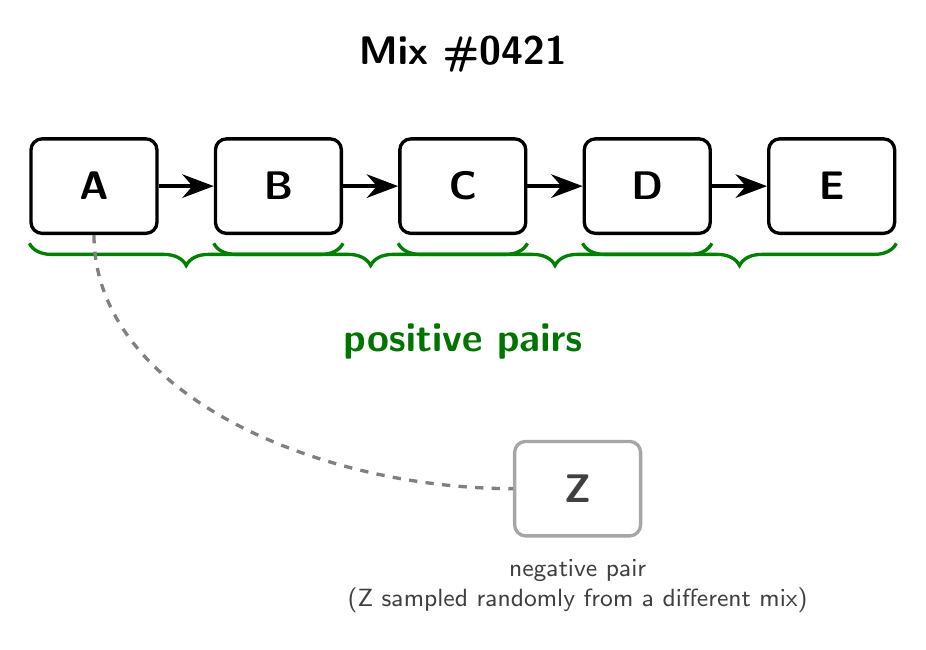
\begin{tikzpicture}[node distance=0.7cm]
  \node[trackbox] (A) {A};
  \node[trackbox, right=of A] (B) {B};
  \node[trackbox, right=of B] (C) {C};
  \node[trackbox, right=of C] (D) {D};
  \node[trackbox, right=of D] (E) {E};

  \draw[flow] (A) -- (B);
  \draw[flow] (B) -- (C);
  \draw[flow] (C) -- (D);
  \draw[flow] (D) -- (E);

  \node[above=0.7cm of C, font=\Large\bfseries] {Mix \#0421};

  \draw[posbrace] ([yshift=-3pt] A.south west) -- ([yshift=-3pt] B.south east);
  \draw[posbrace] ([yshift=-3pt] B.south west) -- ([yshift=-3pt] C.south east);
  \draw[posbrace] ([yshift=-3pt] C.south west) -- ([yshift=-3pt] D.south east);
  \draw[posbrace] ([yshift=-3pt] D.south west) -- ([yshift=-3pt] E.south east);

  \node[below=1.0cm of C, font=\Large\bfseries, color=green!45!black]
    {positive pairs};

  \node[trackbox, draw=gray!70, text=gray!50!black,
        below right=2.6cm and 4.5cm of A] (Z) {Z};
  \draw[negedge] (A.south) .. controls +(0,-2.0cm) and +(-2.5cm,0) .. (Z.west);
  \node[below=0.15cm of Z, font=\small, color=gray!50!black, align=center] {%
    negative pair\\
    (Z sampled randomly from a different mix)};
\end{tikzpicture}

% ============================================================
% ASSET 2 — Model architecture
% ============================================================
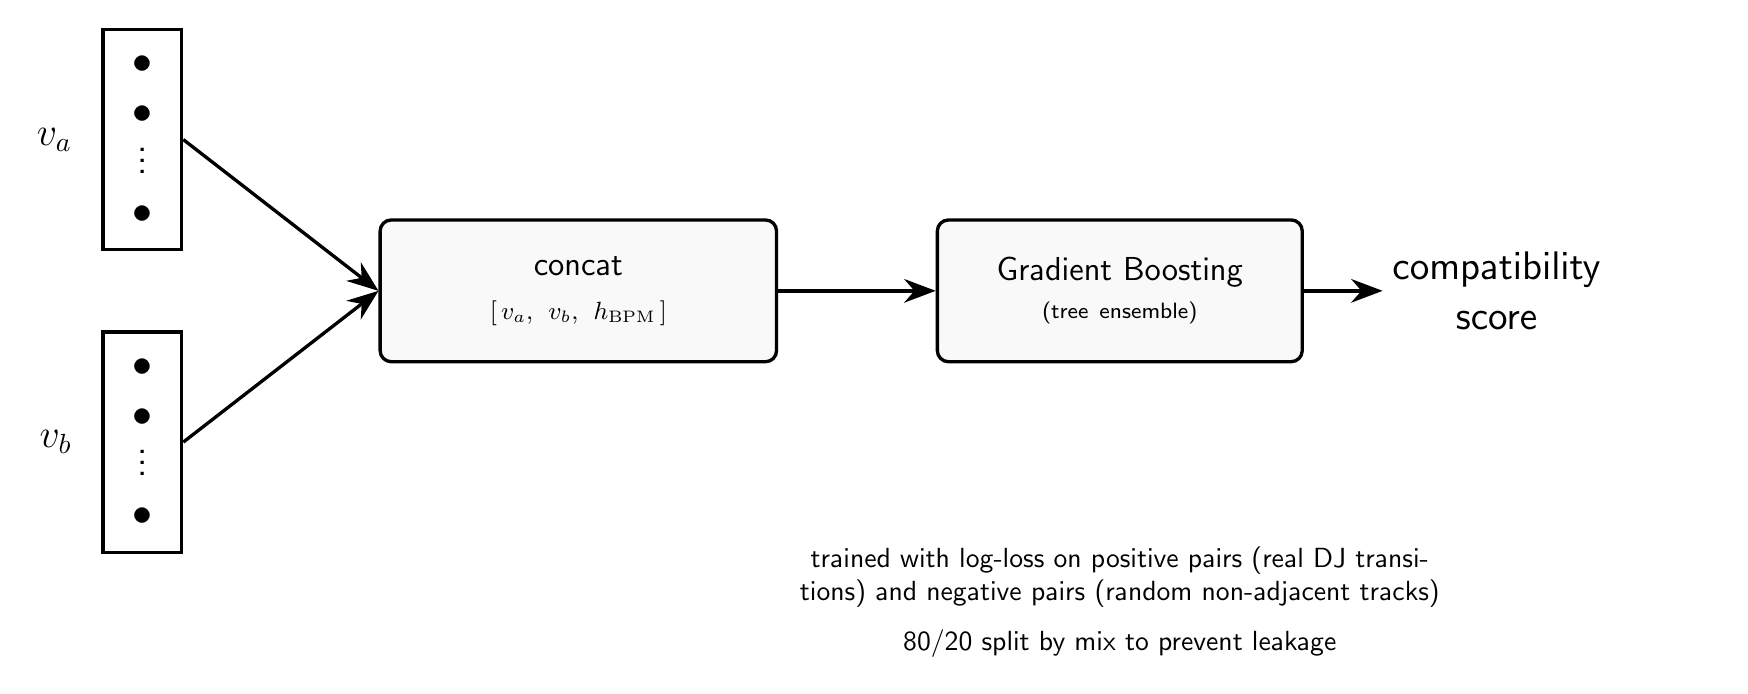
\begin{tikzpicture}[node distance=2cm]
  \node[vector] (va) {$\bullet$\\$\bullet$\\$\vdots$\\$\bullet$};
  \node[left=0.25cm of va, font=\Large] {$v_a$};

  \node[vector, below=1cm of va] (vb) {$\bullet$\\$\bullet$\\$\vdots$\\$\bullet$};
  \node[left=0.25cm of vb, font=\Large] {$v_b$};

  \node[block, right=3cm of $(va)!0.5!(vb)$,
        minimum width=5.0cm, text width=4.8cm] (concat) {%
    concat\\[2pt]
    {\small $[\,v_a,\ v_b,\ h_{\mathrm{BPM}}\,]$}};

  \node[block, right=of concat, minimum width=4.6cm, text width=4.4cm] (mlp) {%
    Gradient Boosting\\
    {\footnotesize (tree ensemble)}};
  \node[right=1.0cm of mlp, font=\Large, align=center] (score) {%
    compatibility\\ score};

  \draw[flow] (va.east) -- (concat.west);
  \draw[flow] (vb.east) -- (concat.west);
  \draw[flow] (concat) -- (mlp);
  \draw[flow] (mlp) -- (score);

  \node[below=2.2cm of mlp, text width=15cm, align=center, font=\normalsize] {%
    trained with log-loss on positive pairs (real DJ transitions) and negative pairs (random non-adjacent tracks)\\[6pt]
    80/20 split by mix to prevent leakage};
\end{tikzpicture}

% ============================================================
% ASSET 3 — Harmonic BPM feature
% ============================================================
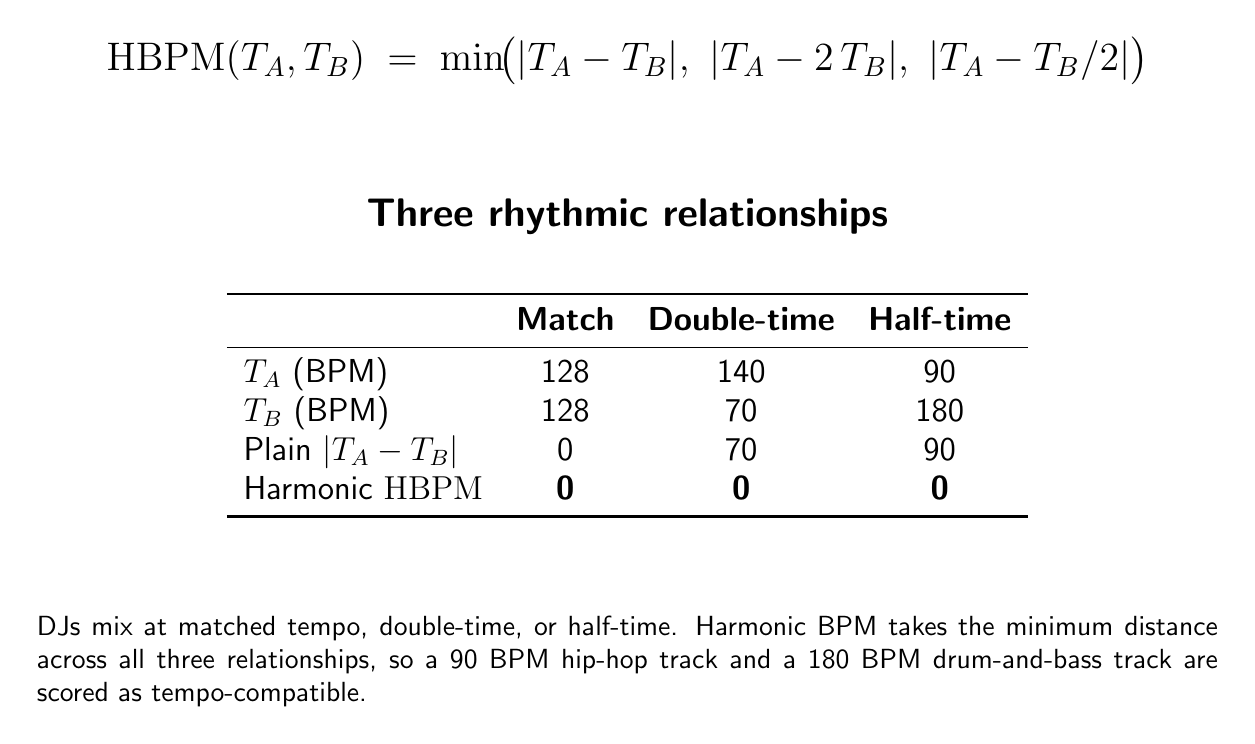
\begin{tikzpicture}[node distance=0.8cm]
  \node[font=\Large] (eq) {%
    $\displaystyle
      \mathrm{HBPM}(T_A, T_B) \;=\;
      \min\!\bigl(
        |T_A - T_B|,\
        |T_A - 2\,T_B|,\
        |T_A - T_B/2|
      \bigr)$};

  \node[below=1.2cm of eq, font=\Large\bfseries] (label) {Three rhythmic relationships};

  \node[below=0.5cm of label, font=\large] (table) {%
    \begin{tabular}{lccc}
      \toprule
        & \textbf{Match} & \textbf{Double-time} & \textbf{Half-time} \\
      \midrule
      $T_A$ (BPM)              & 128        & 140        & 90         \\
      $T_B$ (BPM)              & 128        & 70         & 180        \\
      Plain $|T_A - T_B|$      & 0          & 70         & 90         \\
      Harmonic $\mathrm{HBPM}$ & \textbf{0} & \textbf{0} & \textbf{0} \\
      \bottomrule
    \end{tabular}};

  \node[below=1.0cm of table, text width=15cm, font=\normalsize, align=justify] {%
    DJs mix at matched tempo, double-time, or half-time. Harmonic BPM takes the minimum distance across all three relationships, so a 90 BPM hip-hop track and a 180 BPM drum-and-bass track are scored as tempo-compatible.};
\end{tikzpicture}

% ============================================================
% ASSET 4 — Full pipeline
% ============================================================
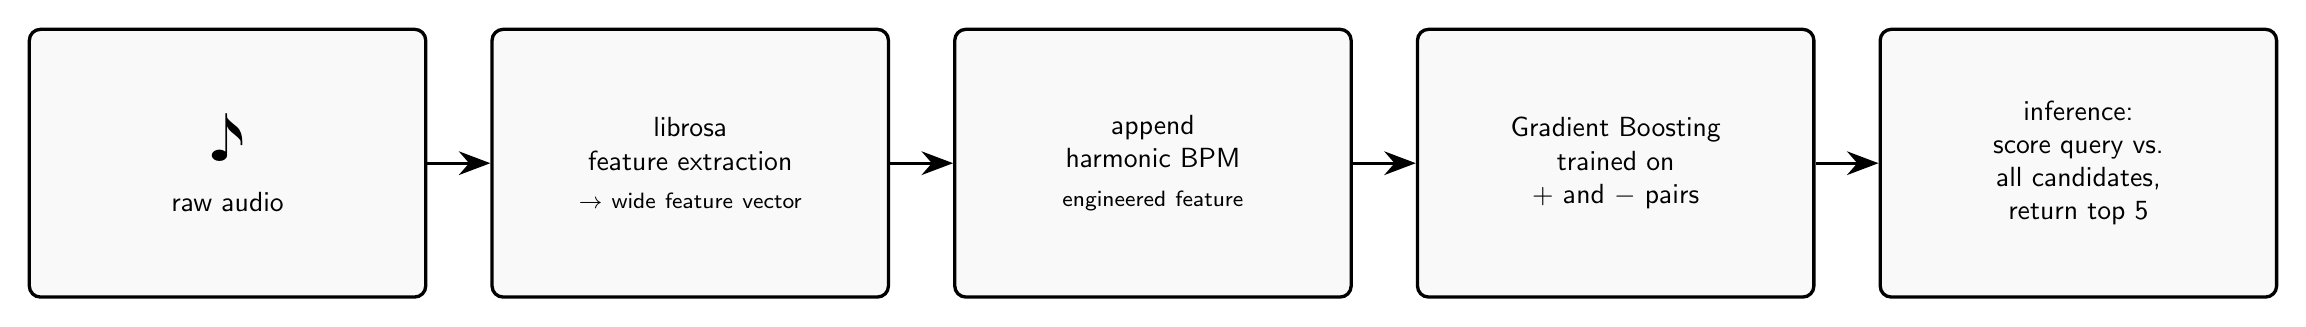
\begin{tikzpicture}[node distance=0.8cm]
  \node[pipestage] (s1) {%
    {\Huge\eighthnote}\\[6pt]
    raw audio};
  \node[pipestage, right=of s1] (s2) {%
    librosa\\
    feature extraction\\[2pt]
    {\footnotesize $\to$ wide feature vector}};
  \node[pipestage, right=of s2] (s3) {%
    append\\
    harmonic BPM\\[2pt]
    {\footnotesize engineered feature}};
  \node[pipestage, right=of s3] (s4) {%
    Gradient Boosting\\
    trained on\\
    $+$ and $-$ pairs};
  \node[pipestage, right=of s4] (s5) {%
    inference:\\
    score query vs.\\
    all candidates,\\
    return top 5};

  \draw[flow] (s1) -- (s2);
  \draw[flow] (s2) -- (s3);
  \draw[flow] (s3) -- (s4);
  \draw[flow] (s4) -- (s5);
\end{tikzpicture}

% ============================================================
% ASSET 5 — Inference behavior
% ============================================================
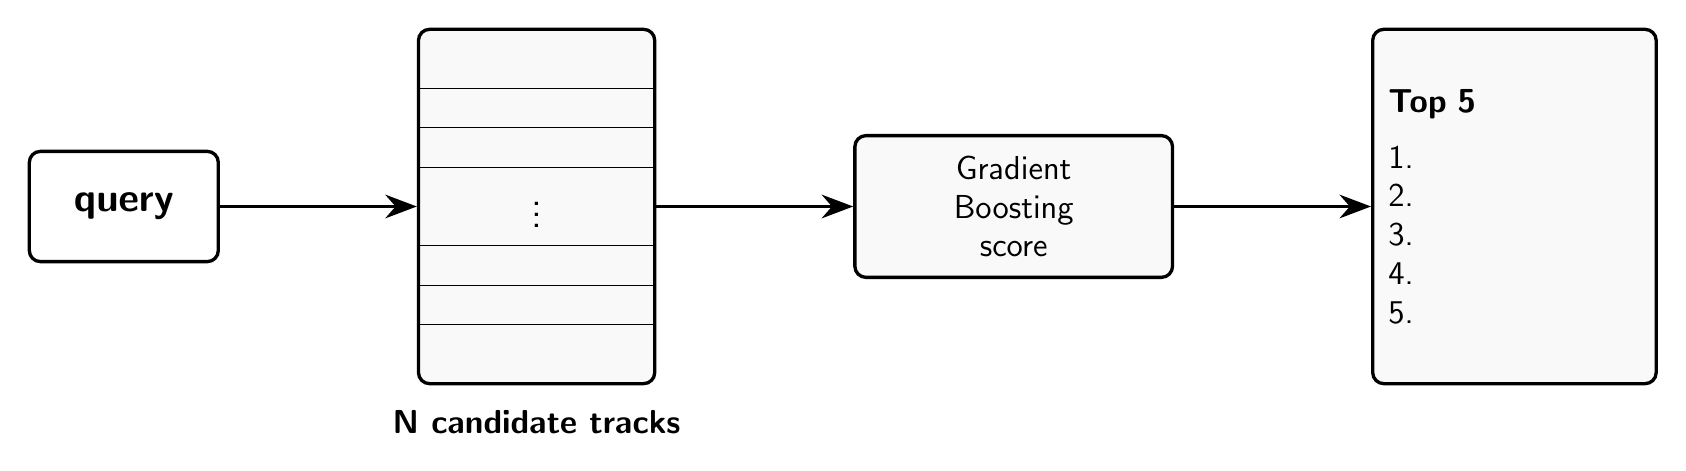
\begin{tikzpicture}
  \node[trackbox, minimum width=2.4cm, minimum height=1.4cm] (q) {query};

  \node[draw, very thick, rounded corners,
        minimum width=3cm, minimum height=4.5cm,
        right=2.5cm of q, fill=gray!5] (lib) {};
  \foreach \yy in {-1.5,-1.0,-0.5,0.5,1.0,1.5} {
    \draw ([yshift=\yy cm] lib.west) -- ([yshift=\yy cm] lib.east);
  }
  \node[font=\Large] at (lib) {$\vdots$};
  \node[below=0.2cm of lib, font=\large\bfseries, align=center]
    {N candidate tracks};

  \node[block, right=2.5cm of lib, minimum width=4.0cm, text width=3.8cm] (mlp) {%
    Gradient\\ Boosting\\ score};

  \node[draw, very thick, rounded corners, fill=gray!5,
        right=2.5cm of mlp, font=\large, align=left,
        minimum width=3.6cm, minimum height=4.5cm,
        text width=3.2cm] (top5) {%
    \textbf{Top 5}\\[6pt]
    1.\\
    2.\\
    3.\\
    4.\\
    5.};

  \draw[flow] (q) -- (lib);
  \draw[flow] (lib) -- (mlp);
  \draw[flow] (mlp) -- (top5);
\end{tikzpicture}

% ============================================================
% ASSET 6 — Train / Test split
% Two stacked panels, pink-tinted to match the existing poster
% style. Each panel shows two example tracks (v_a, v_b) feeding the
% Gradient Boosting model. Training side fits to labels; testing
% side produces a score against held-out pairs.
% ============================================================
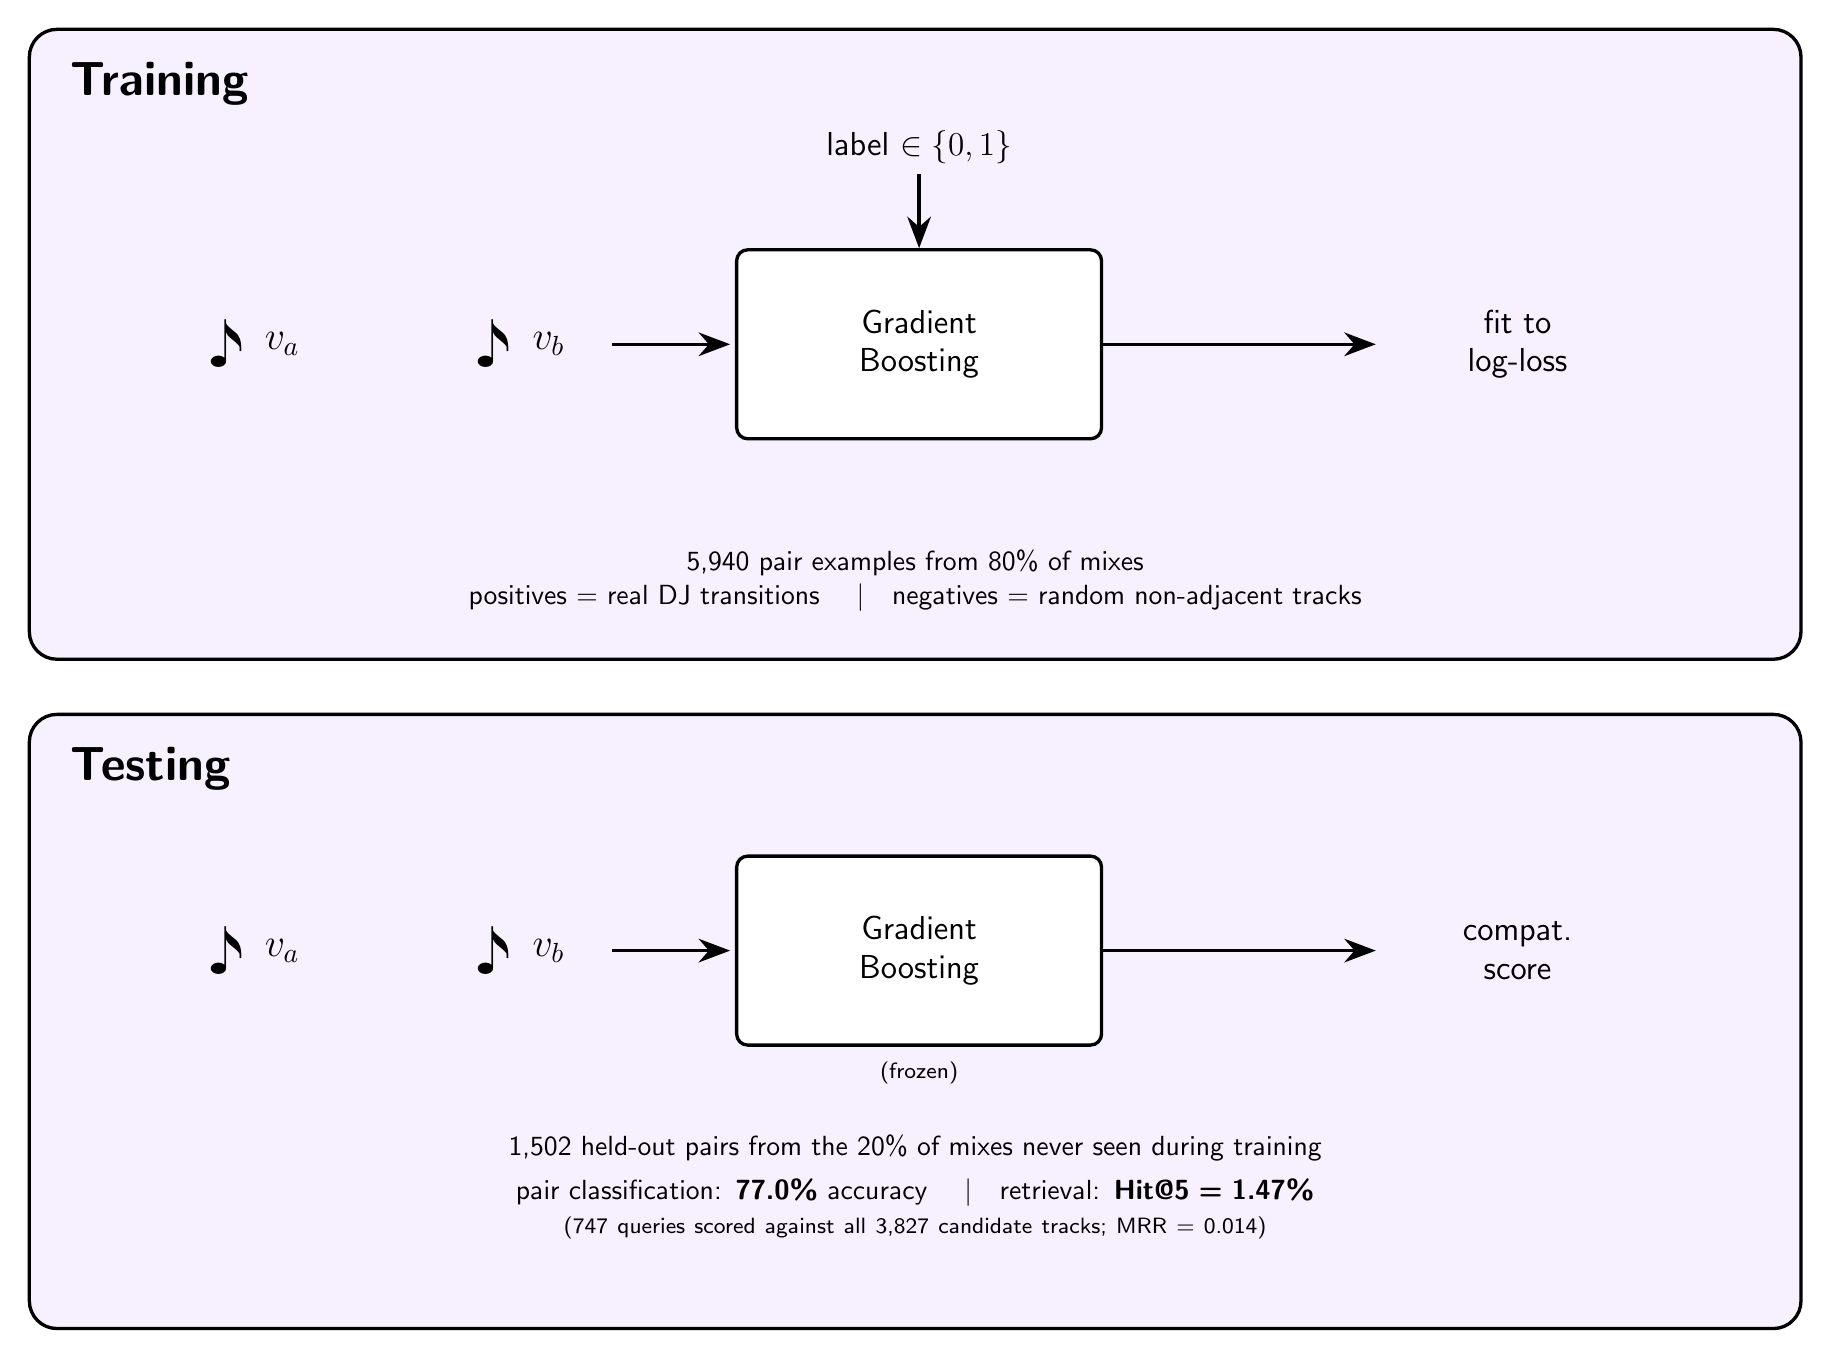
\begin{tikzpicture}
  % ===== Training panel =====
  \fill[posterbg, rounded corners=10pt] (-0.5, -7.0) rectangle (22, 1.0);
  \draw[very thick, rounded corners=10pt] (-0.5, -7.0) rectangle (22, 1.0);

  \node[font=\LARGE\bfseries, anchor=north west] at (-0.1, 0.7) {Training};

  \node[font=\Huge] (tn_a) at (2.0, -3.0) {\eighthnote};
  \node[right=0pt of tn_a, font=\Large] {$v_a$};
  \node[font=\Huge] (tn_b) at (5.4, -3.0) {\eighthnote};
  \node[right=0pt of tn_b, font=\Large] {$v_b$};

  \draw[flow] (6.9, -3.0) -- (8.4, -3.0);

  \node[draw, very thick, rounded corners, fill=white,
        minimum width=4.6cm, minimum height=2.4cm, text width=4.4cm,
        font=\large, align=center] (tmodel) at (10.8, -3.0) {%
    Gradient\\ Boosting};

  \draw[flow] (tmodel.east) -- (16.6, -3.0);

  \node[font=\large, align=center] at (18.4, -3.0) {fit to\\ log-loss};

  % label arrow into model from above
  \node[font=\large, align=center] (lbl) at (10.8, -0.5) {label $\in \{0, 1\}$};
  \draw[flow] (lbl.south) -- (tmodel.north);

  \node[font=\normalsize, align=center, text width=22cm] at (10.75, -6.0) {%
    5{,}940 pair examples from 80\% of mixes\\
    positives = real DJ transitions \quad\textbar\quad negatives = random non-adjacent tracks};

  % ===== Testing panel =====
  \fill[posterbg, rounded corners=10pt] (-0.5, -15.5) rectangle (22, -7.7);
  \draw[very thick, rounded corners=10pt] (-0.5, -15.5) rectangle (22, -7.7);

  \node[font=\LARGE\bfseries, anchor=north west] at (-0.1, -8.0) {Testing};

  \node[font=\Huge] (sn_a) at (2.0, -10.7) {\eighthnote};
  \node[right=0pt of sn_a, font=\Large] {$v_a$};
  \node[font=\Huge] (sn_b) at (5.4, -10.7) {\eighthnote};
  \node[right=0pt of sn_b, font=\Large] {$v_b$};

  \draw[flow] (6.9, -10.7) -- (8.4, -10.7);

  \node[draw, very thick, rounded corners, fill=white,
        minimum width=4.6cm, minimum height=2.4cm, text width=4.4cm,
        font=\large, align=center] (smodel) at (10.8, -10.7) {%
    Gradient\\ Boosting};
  \node[font=\footnotesize, below=2pt of smodel] {(frozen)};

  \draw[flow] (smodel.east) -- (16.6, -10.7);

  \node[font=\large, align=center] at (18.4, -10.7) {compat.\\ score};

  \node[font=\normalsize, align=center, text width=20cm] at (10.75, -13.7) {%
    1{,}502 held-out pairs from the 20\% of mixes never seen during training\\[4pt]
    pair classification: \textbf{77.0\%} accuracy \quad\textbar\quad retrieval: \textbf{Hit@5 = 1.47\%}\\
    {\footnotesize (747 queries scored against all 3{,}827 candidate tracks; MRR = 0.014)}};
\end{tikzpicture}

\end{document}
